% small.tex
\documentclass{beamer}
\usepackage{graphicx}                           % Includes packages for the LaTeX document.
%\usepackage[left=1.5in,top=1.25in,bottom=1.25in,right=1.25in]{geometry} % Sets the proper margins.
\usepackage{mathptmx}
\usetheme{default}%\usepackage{cite}
\usecolortheme{dove}
\useinnertheme{rounded}
\usepackage{amssymb}
\usepackage{amsmath}
\usepackage{gensymb}

\usepackage{tikz}
\usetikzlibrary{calc,shapes,arrows,positioning,decorations.pathreplacing,decorations.pathmorphing,matrix,shapes.symbols}
\setbeamertemplate{navigation symbols}{}%remove navigation symbols
\title{Face Recognition and Tracking}
\subtitle{using OpenCV, Python, and cheap hardware}
\author{Steve Burt}

\begin{document}

\begin{frame}[plain]
\begin{center}
\LARGE Simple 2-axis face tracking\\
\LARGE with cheap hardware\\
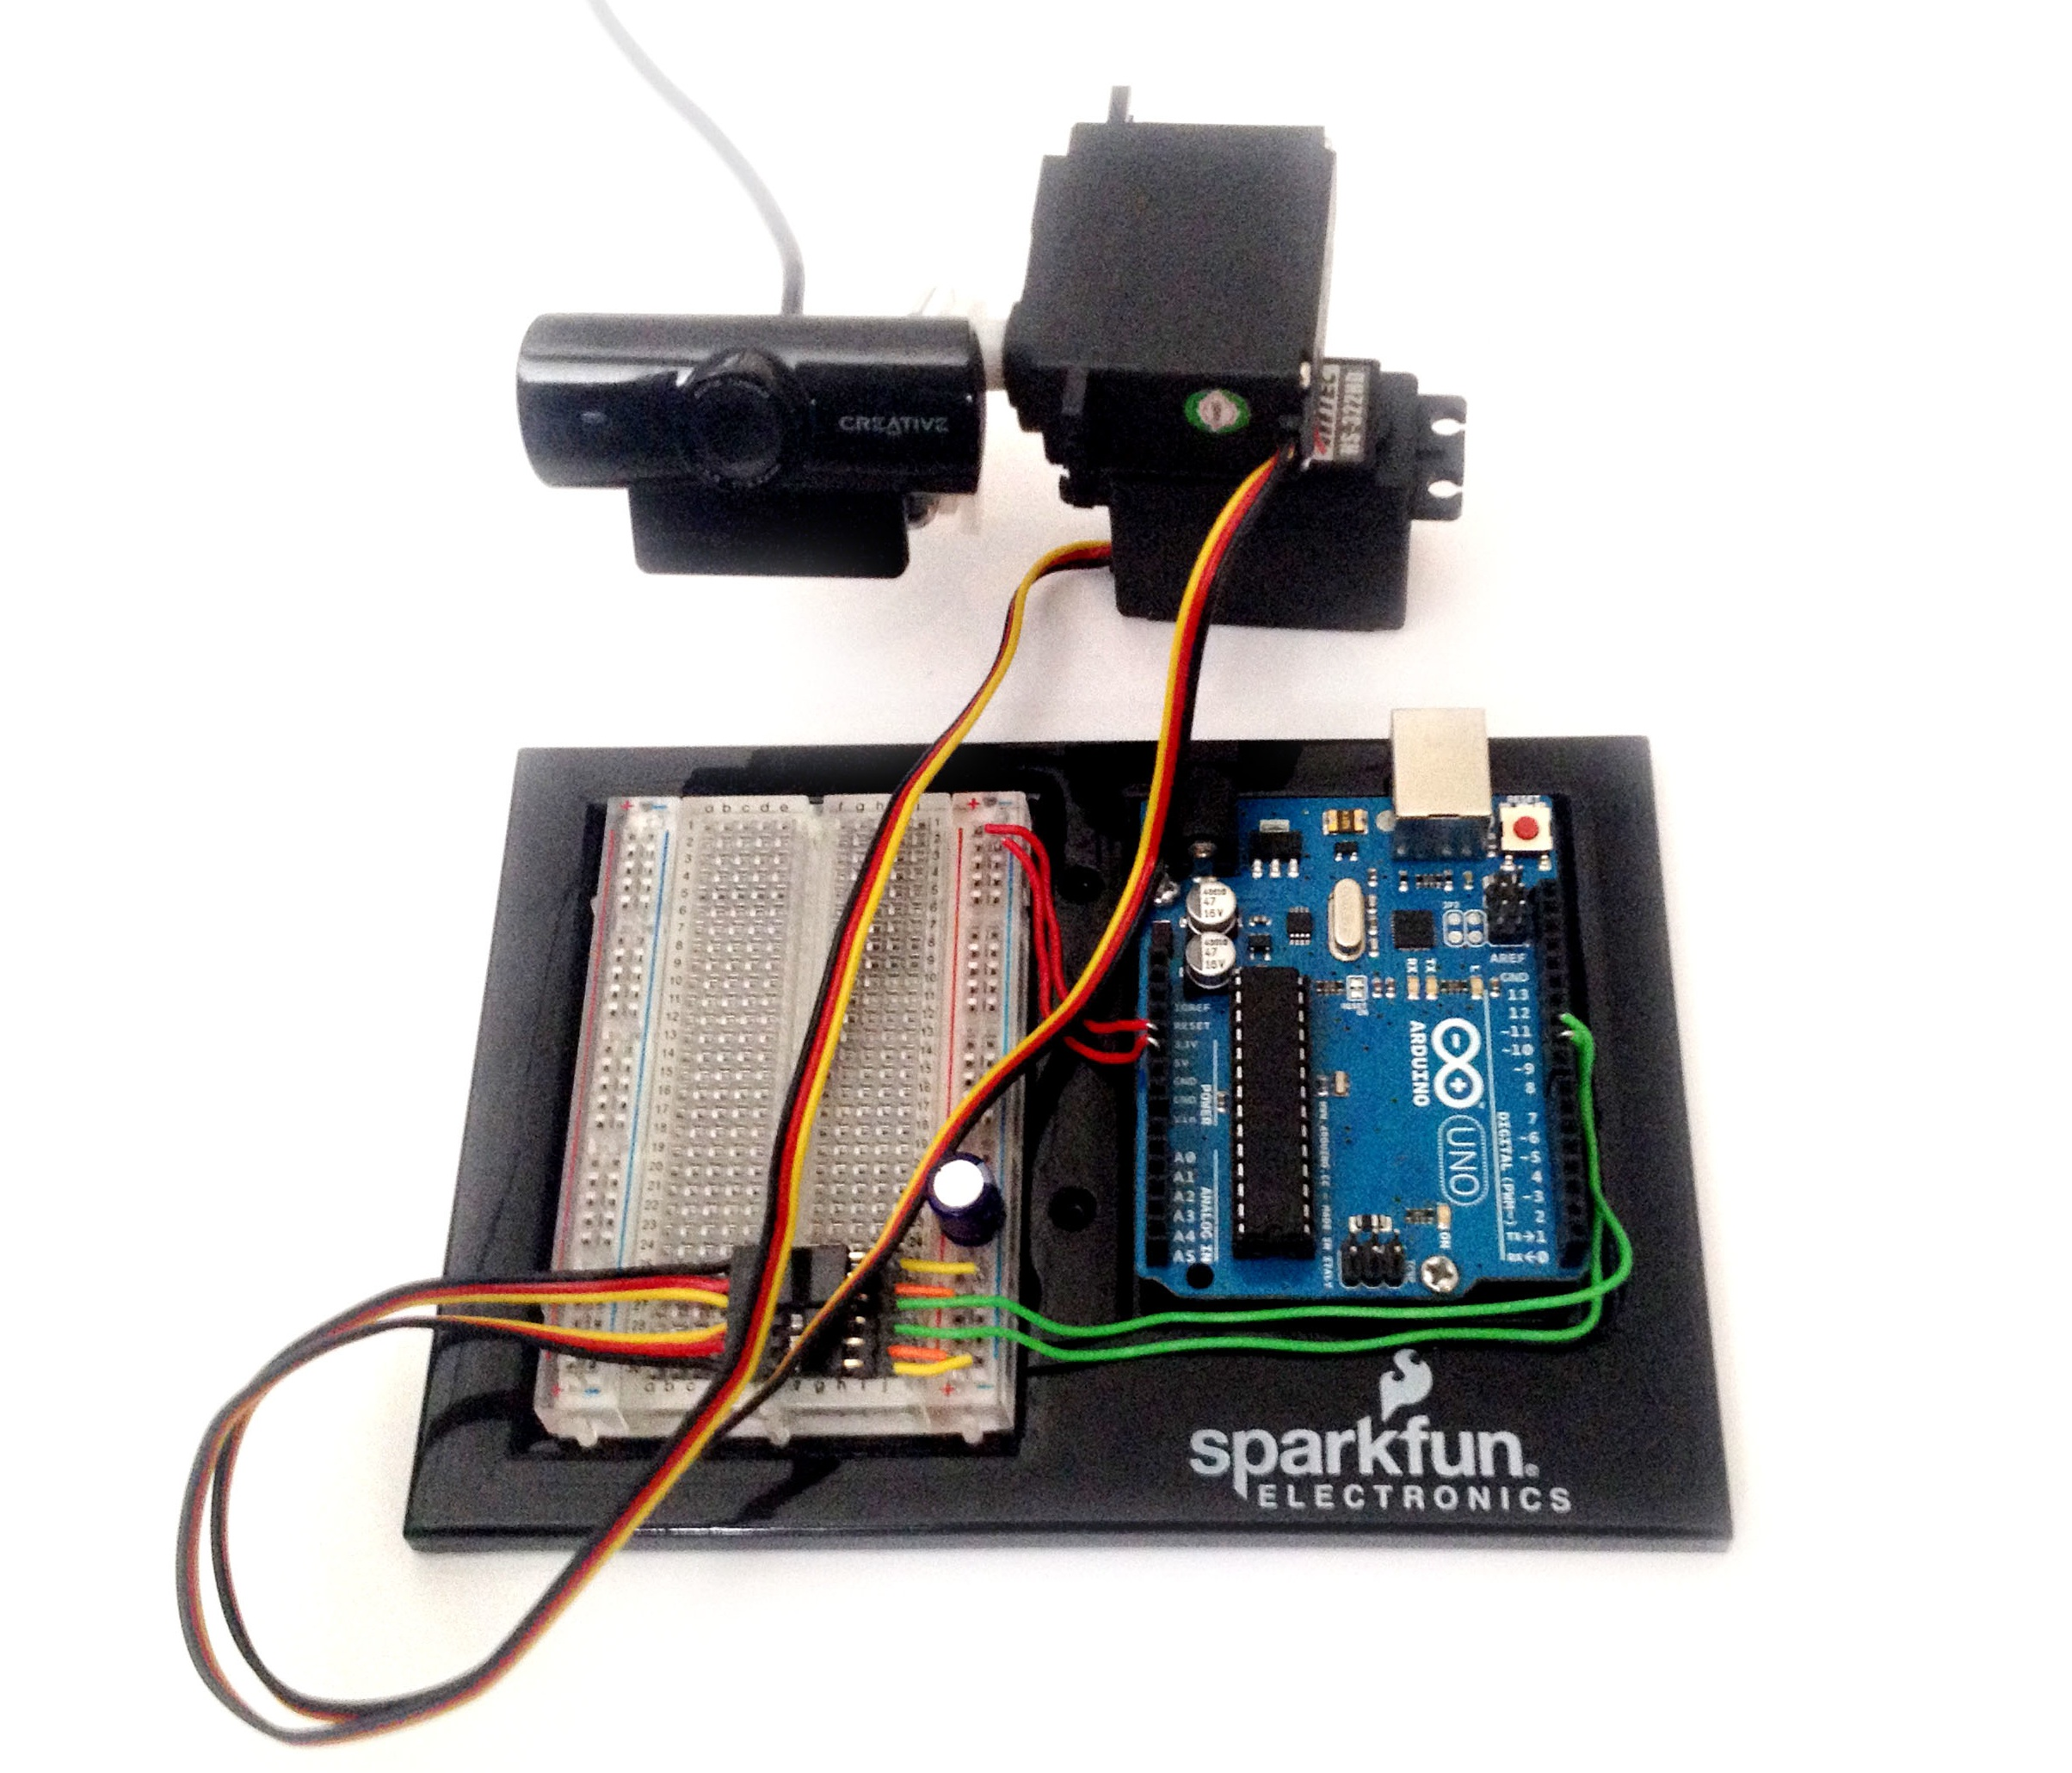
\includegraphics[width=3in]{board}
\Large Steven Burt 
\end{center}
\end{frame}
\begin{frame}{Architecture}

\centering
\parbox{.45\textwidth}{  Data Flow\\ \\
\includegraphics[width=\linewidth]{meta-1}}\parbox{.5\textwidth}{ State Machine\\\includegraphics[width=\linewidth]{sm}}\\
\end{frame}
\begin{frame}{Details}

\begin{columns}
  \begin{column}{0.7\textwidth}
\begin{itemize}
  \item Face detection with Haar classifier, using OpenCV
  \item PyQt GUI
\item \$9 RC servos
\item AtMEGA328P for servo interface
\item \$10 Webcam
\end{itemize}
\end{column}
\begin{column}{.3\textwidth}
\begin{figure}
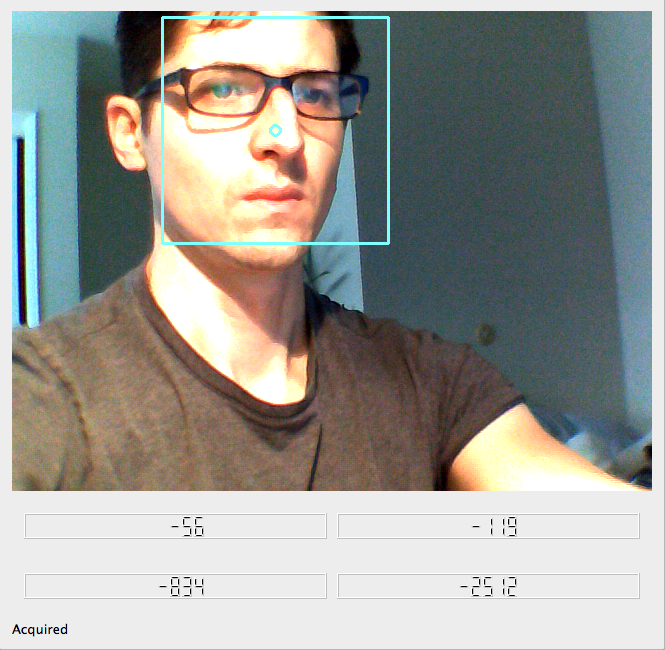
\includegraphics[width=1in]{facetrack2d}
\end{figure}

\end{column}
\end{columns}
\begin{columns}
  \begin{column}{2in}
\begin{figure}
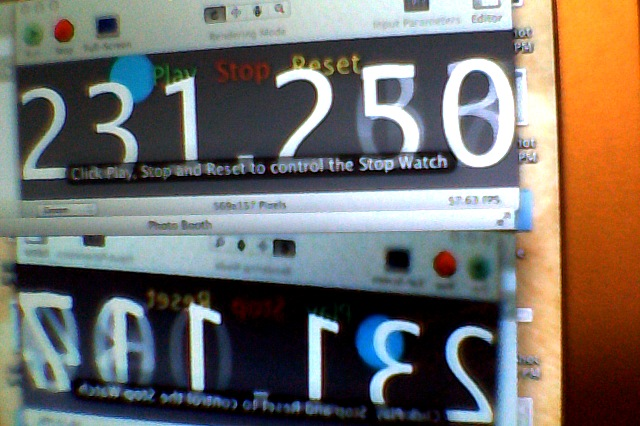
\includegraphics[width=1.5in]{latency}
\end{figure}
  \end{column}
\begin{column}{.6\textwidth}
\textbf{Control Issues:}
\begin{itemize}
\item Webcam has ~200 msec latency
\item Face detection adds about 50msec
\item Bad for feedback control!
\end{itemize}
Latency compensation via control signal feed-back
\end{column}
\end{columns}
\end{frame}

\begin{frame}{Control loop}

\tikzstyle{block} = [draw, rectangle, 
    minimum height=3em, minimum width=6em]
\tikzstyle{sum} = [draw, fill=gray!20, circle, node distance=1cm]
\tikzstyle{input} = [coordinate]
\tikzstyle{output} = [coordinate]
\tikzstyle{pinstyle} = [pin edge={to-,thin,black}]

% The block diagram code is probably more verbose than necessary
\begin{tikzpicture}[auto, node distance=2cm,>=latex']
    % We start by placing the blocks
   	\node [input, name=input] {};
 	\node [sum, right of=input] (sum) {};
  	 \node [block, right of=sum] (controller) {Controller};

	\node[sum, right of = controller, node distance = 3cm](newsum){};
    \draw [->] (controller) -- node[near start,name=u] {$u$} (newsum);
%
     \node [block, right of=newsum, node distance=2cm] (system) {System};
 \draw[->](newsum) -- node[name=upr]{$u*$}(system);
%	
    \node [output, right of=system] (output) {};
  \node [block, below of =controller, fill=gray!30, node distance = 3.5cm] (latency) {Measurement Latency};
	\node[block,below of =system, node distance =3.5cm](measurement){Measurement};
    % Once the nodes are placed, connecting them is easy. 
    \draw [draw,->] (input) -- node {$r$} (sum);
    \draw [->] (sum) -- node {$e$} (controller);
    \draw [->] (system) -- node [name=y] {$y$}(output);
   \draw [->] (y) |- (measurement);
	\draw[->](measurement) -- (latency);

\node [block, fill=gray!30, below of = u, node distance = 1.5cm](sd){Input Delay};
\draw[->](u) -- (sd);
\draw[->](sd)-| node[pos = 0.99]{$-$} (newsum);
    \draw [->] (latency) -| node[pos=0.99] {$-$} 
       node [near end] {$y_m$} (sum);

\draw[->, style=dotted](latency) -- node{ Match } (sd);

\end{tikzpicture} 


\end{frame}
\end{document}